\chapter{Introduction}

%\begin{figure}
%\centerline{
%	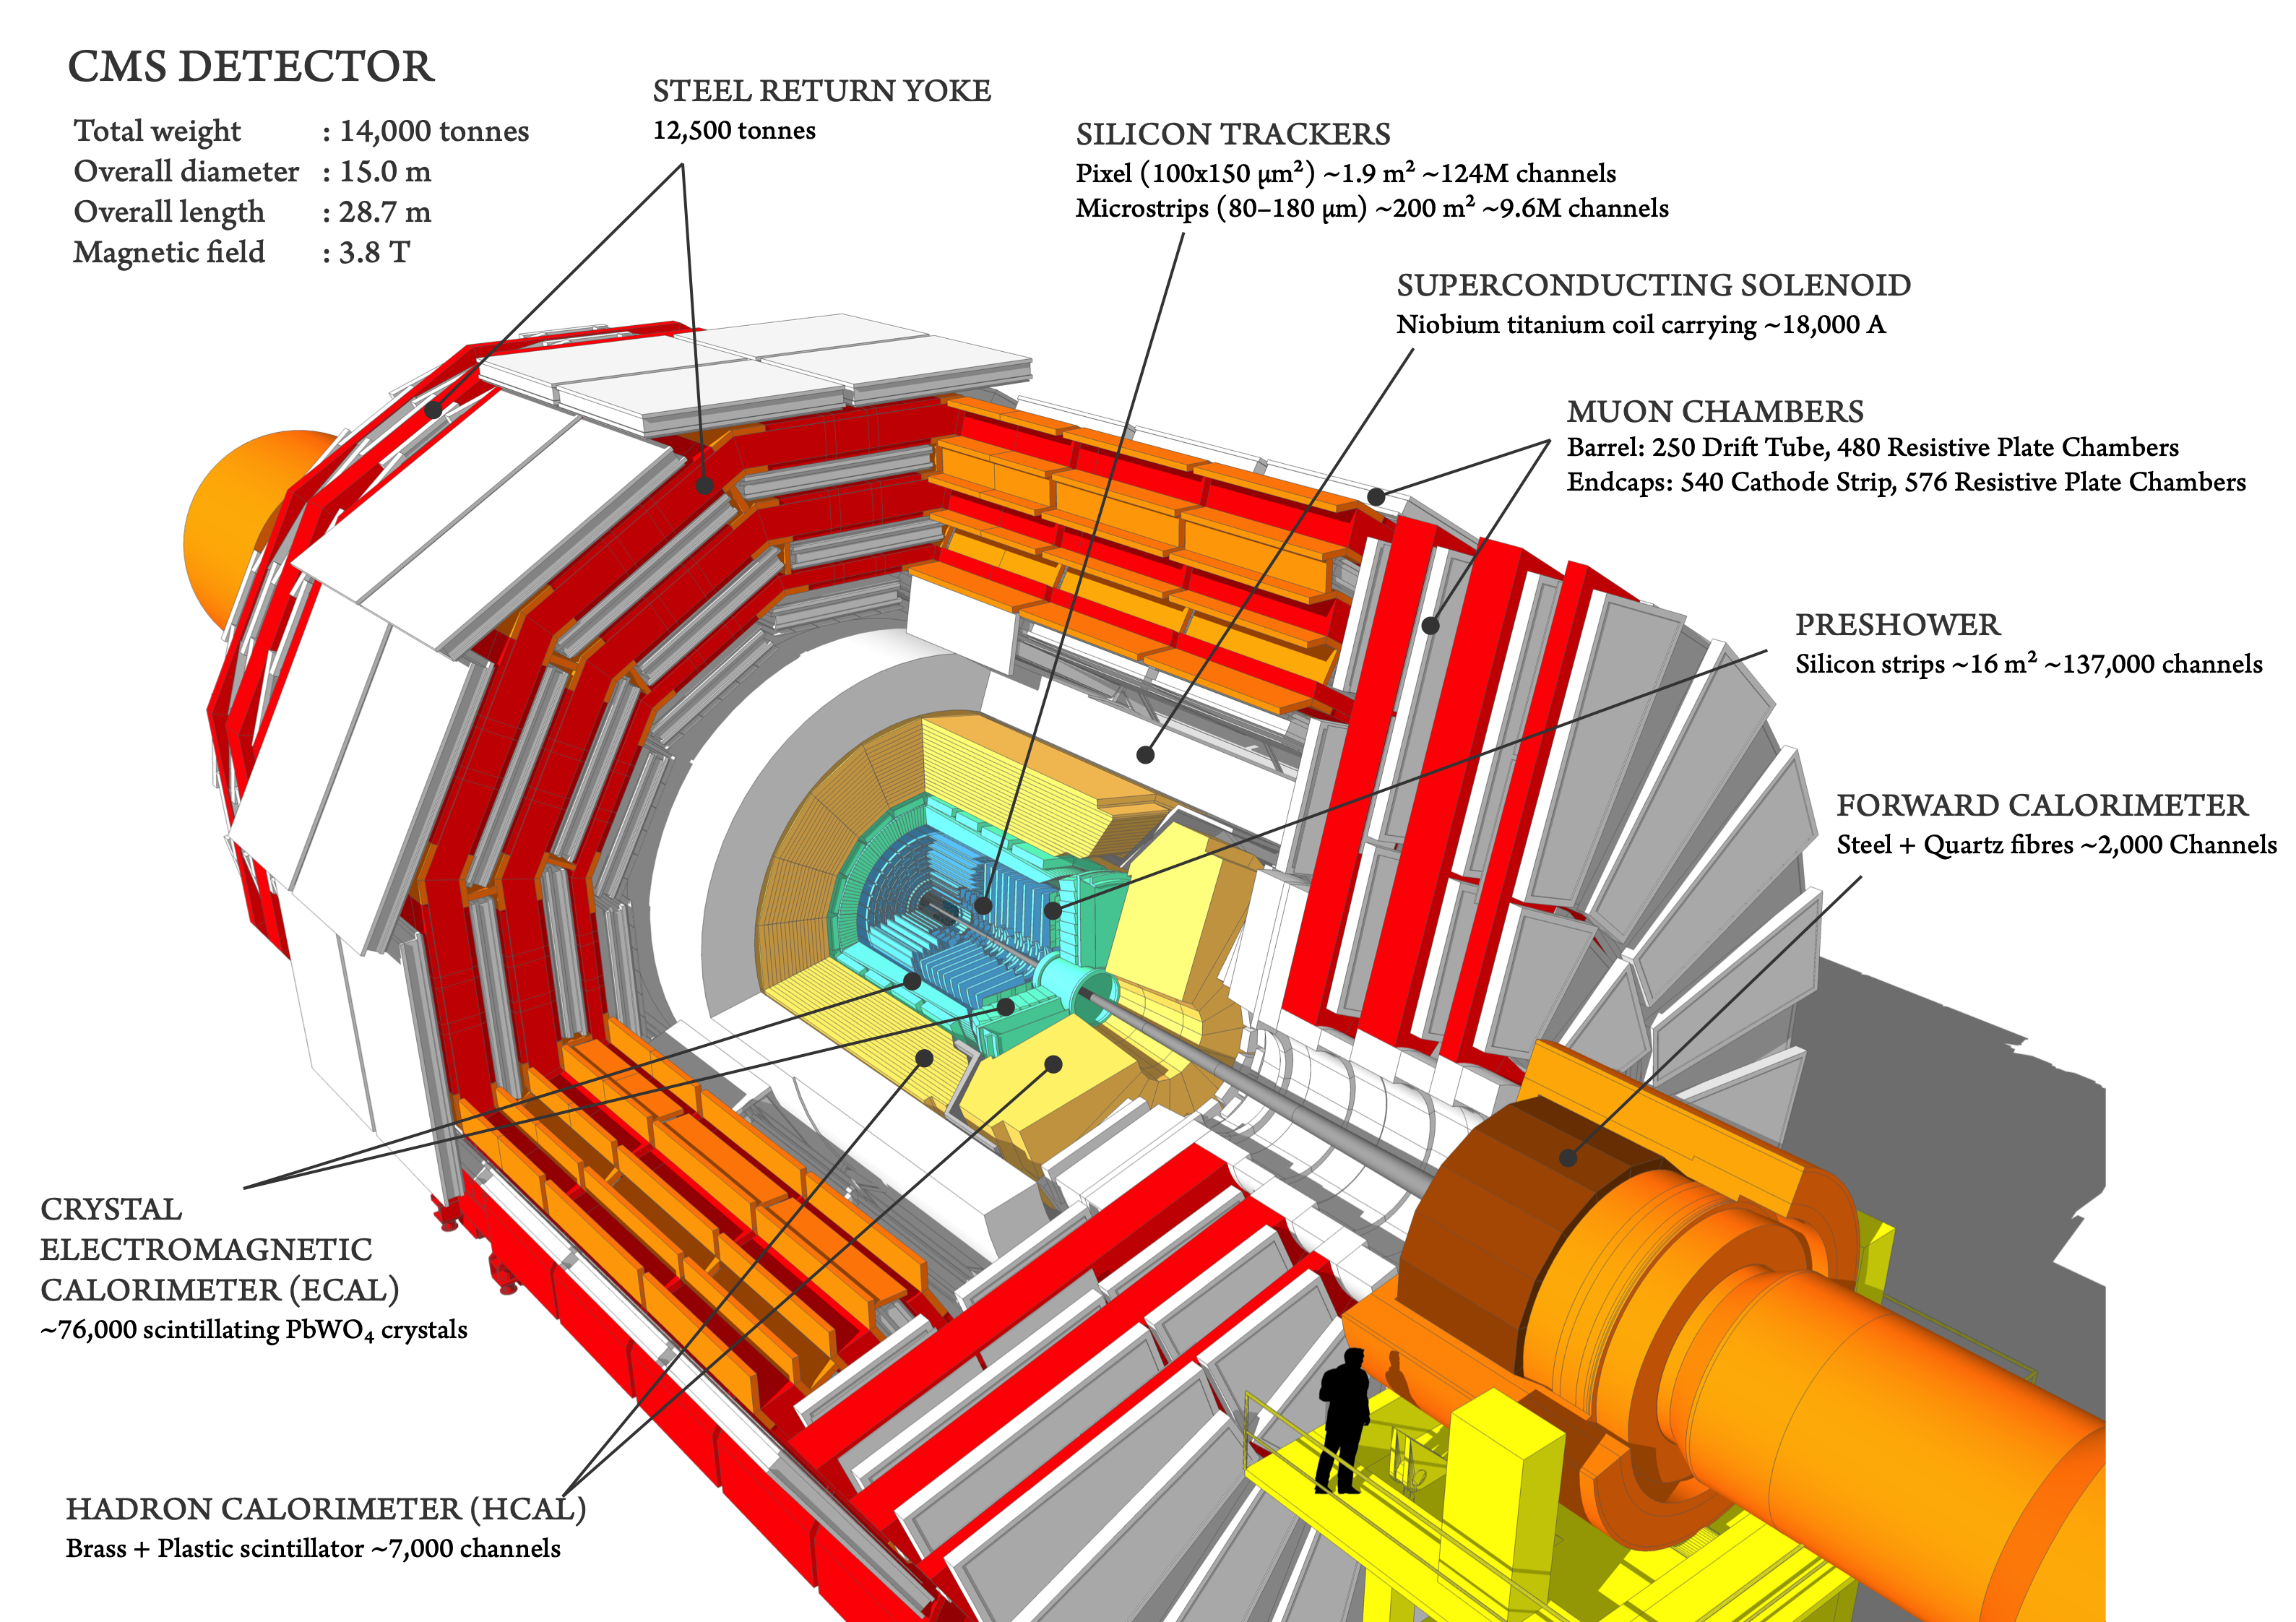
\includegraphics[width=0.75\paperwidth]{cms_160312_06b}}
%	\caption{Cutaway diagram of the CMS detector \cite{Sakuma_2014}}

%\end{figure}

%\begin{figure}
%\centerline{
%	\includegraphics[width=0.75\paperwidth]{CCC-v2019-final-white}}
%	\caption{CERN Accelerators complex \cite{Mobs:2684277}}
%\end{figure}





\section{CERN and the LHC}

\textit{luminosity} value of $10^{34}$ $cm^{-2}$ $s^{-1}$. This value is a measurement of the number of collisions that can be produced in a detector per $cm^2$ and per second.

\section{CMS}


\section{CMS Trigger System}

The first level (L1) of this system restricts the output rate to 100 kHz, the upper limit imposed by the CMS readout electronics. The second level (HLT), implemented in software, further refines this stream, selecting an average rate of 400 Hz for offline event storage and certification \cite{Khachatryan_2017}.
